\section{Porównanie laserów}
\begin{figure}
\center
  \includegraphics[scale=0.30]{plot_common/plot_eff.eps}
  \label{rys1}
  \caption{Wykres sprawności różniczkowej w funkcji prądu oraz mocy wejściowej.}
\end{figure}
\begin{figure}
\center
  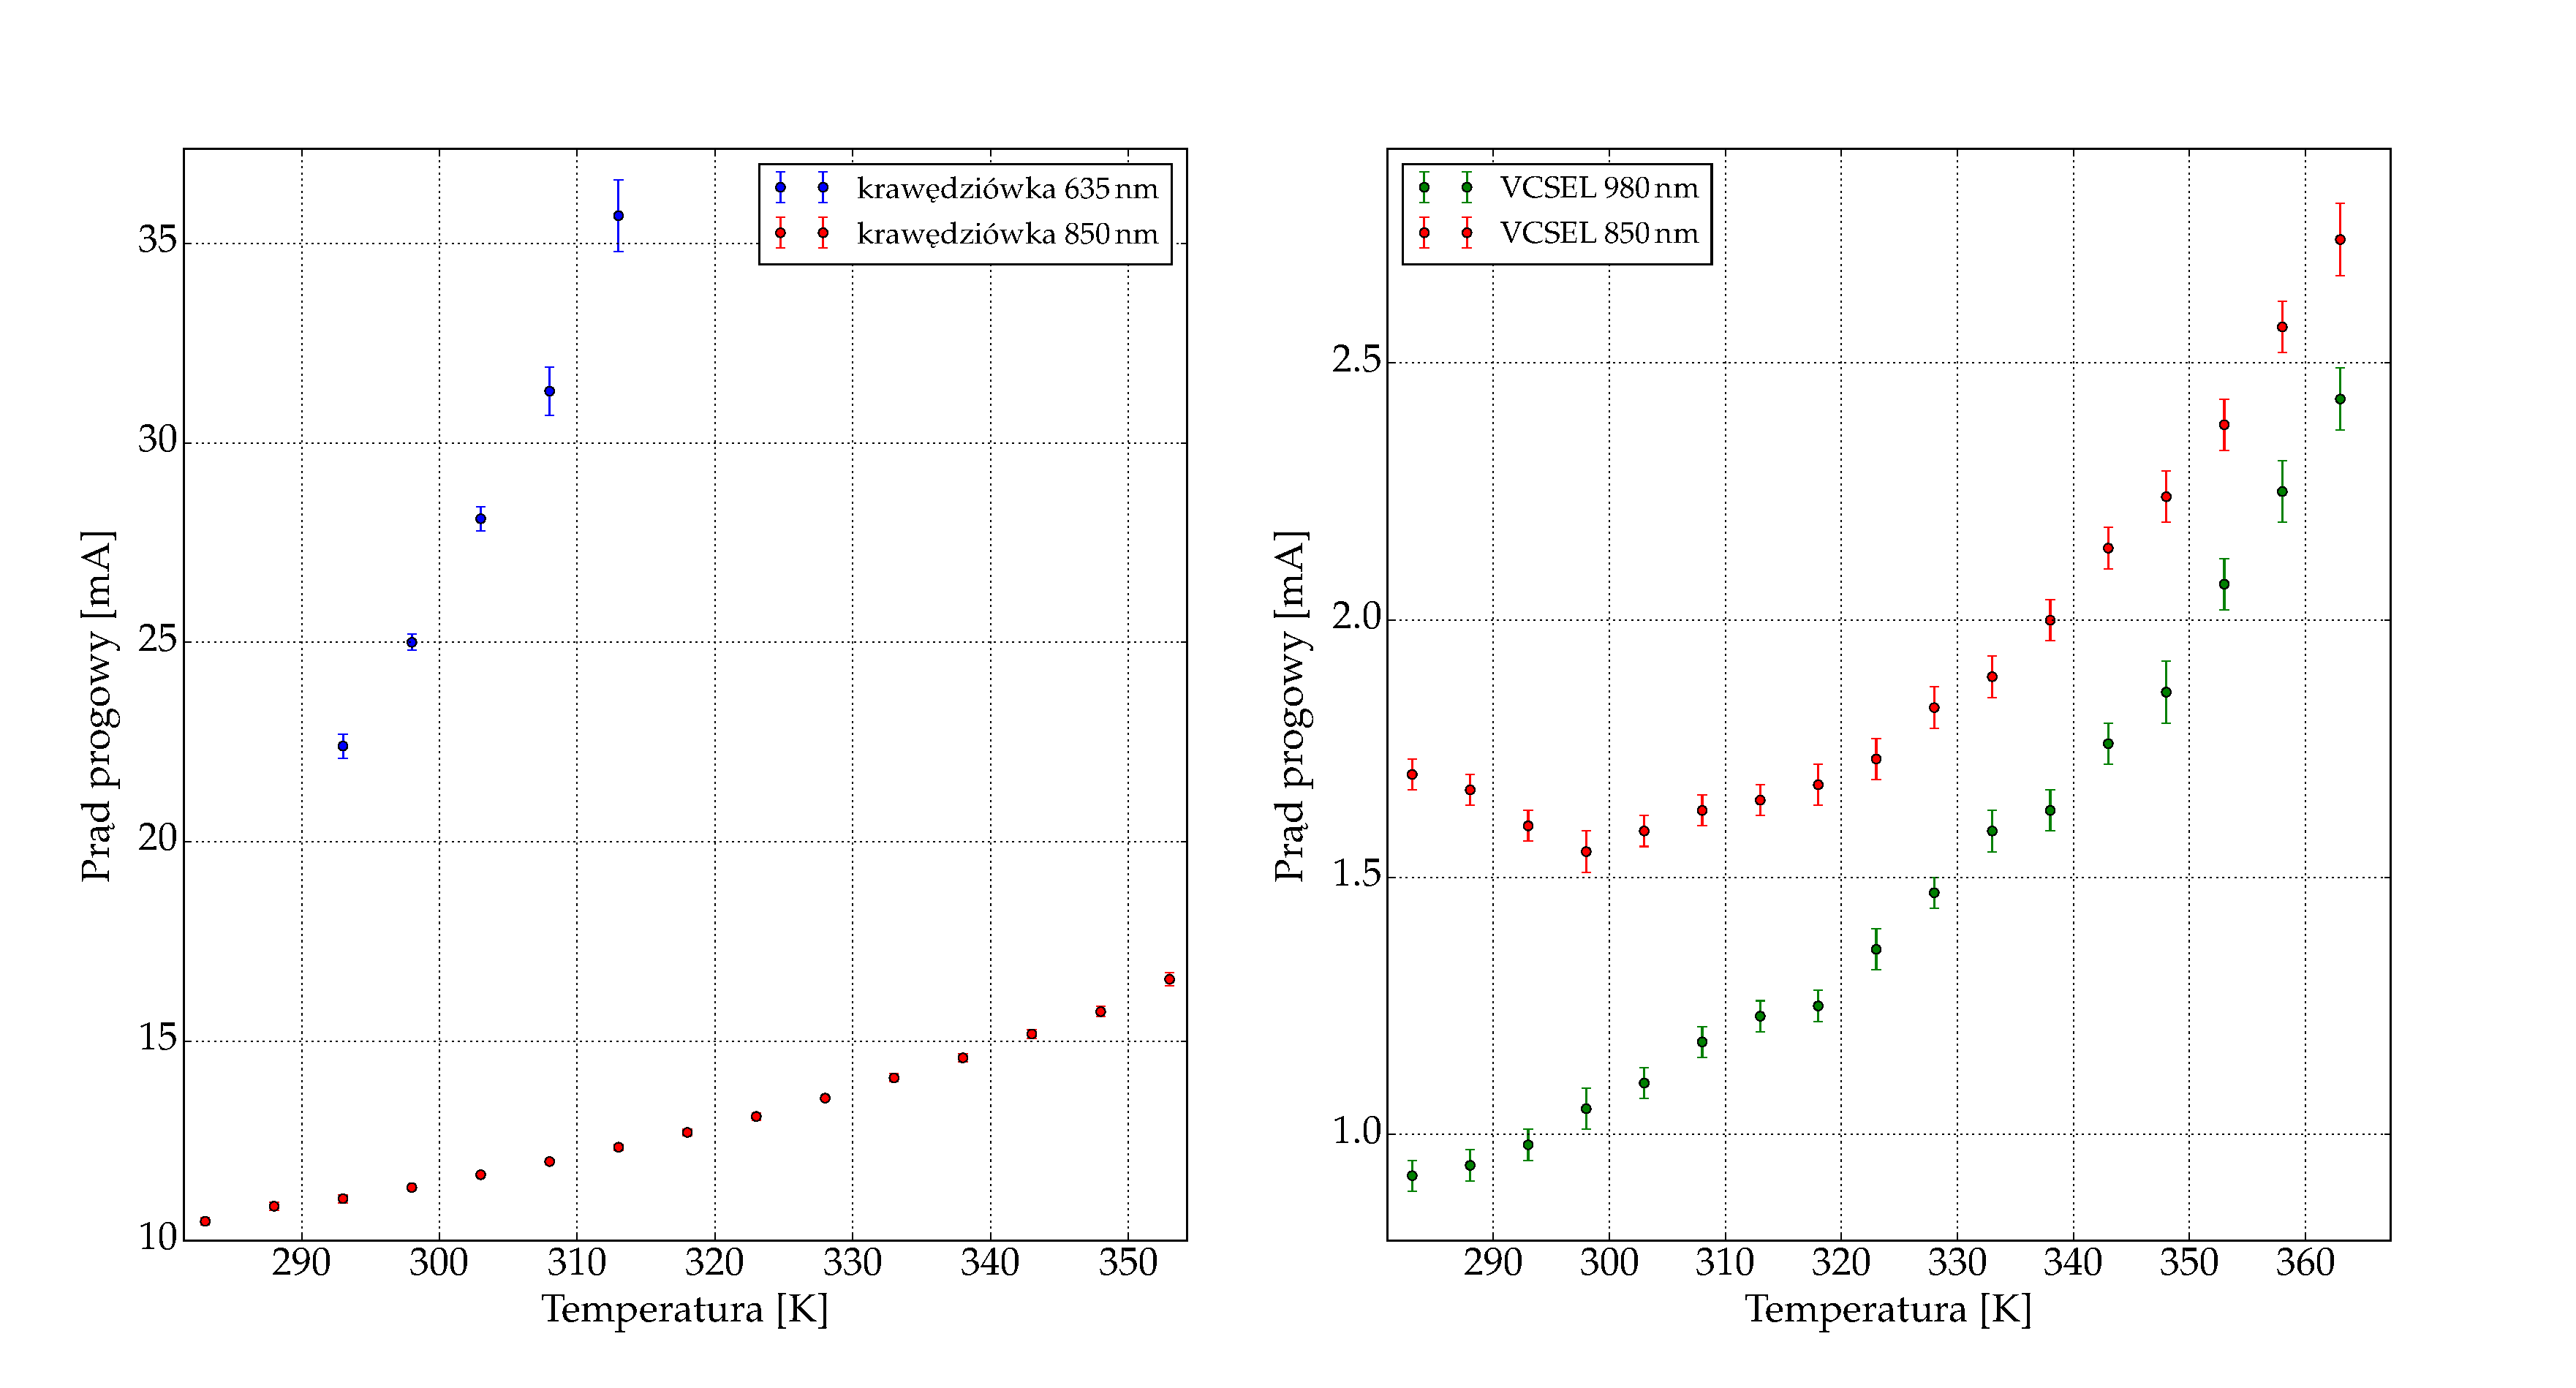
\includegraphics[scale=0.30]{plot_common/plot_temp_i_th.eps}
  \label{rys1}
  \caption{Wykres prądu progowego od temperatury.}
\end{figure}
\begin{figure}
\center
  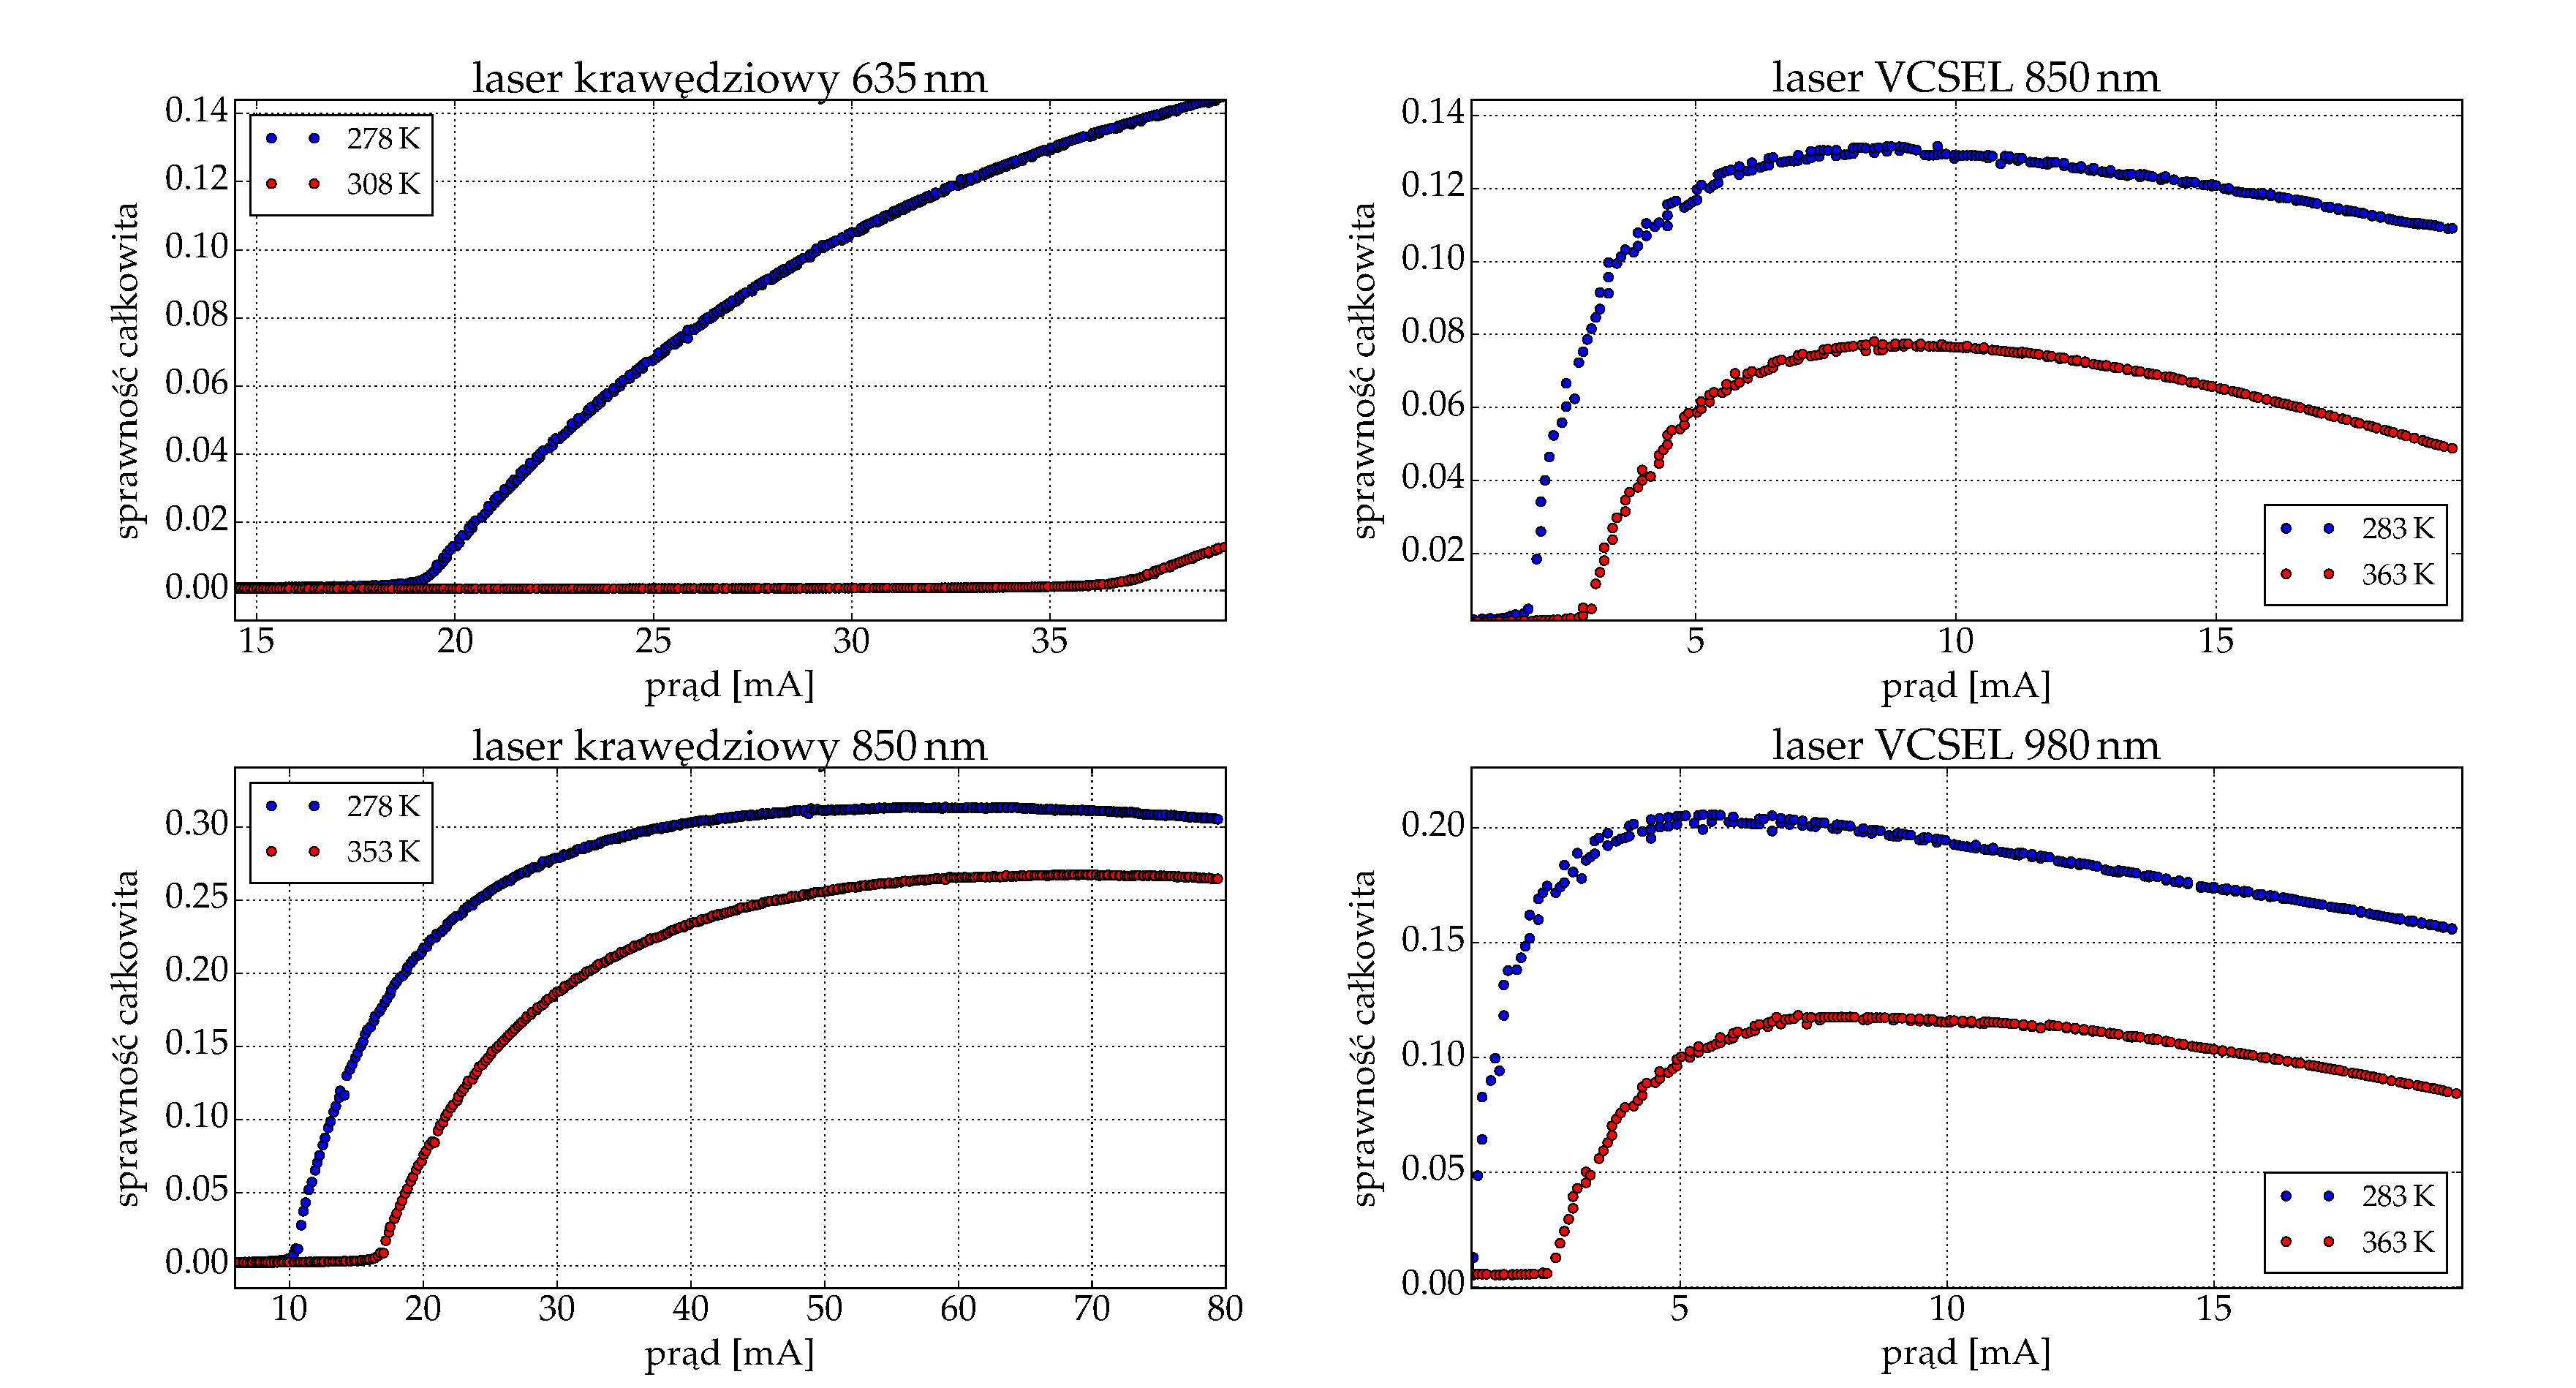
\includegraphics[scale=0.30]{plot_common/plot_wall_eff.eps}
  \label{rys1}
  \caption{Wykres sprawności całkowitej w funkcji prądu.}
\end{figure}
Analizując pomiary dla 4 laserów które przeprowadziłem, można wyciągnąć nastepujące wnioski:
\begin{itemize}
\item Sprawność różniczkowa laserów krawędziowych w funkcji zarówno prądu i mocy wejściowej jest większa.
\item Prąd progowy dla laserów krawędziowych jest większy od prądu progowego dla laserów VCSEL.
\end{itemize}